% Datapath block diagram. Build with:  pdflatex datapath.tex
\documentclass[tikz,border=6pt]{standalone}
\usetikzlibrary{arrows.meta}
\begin{document}
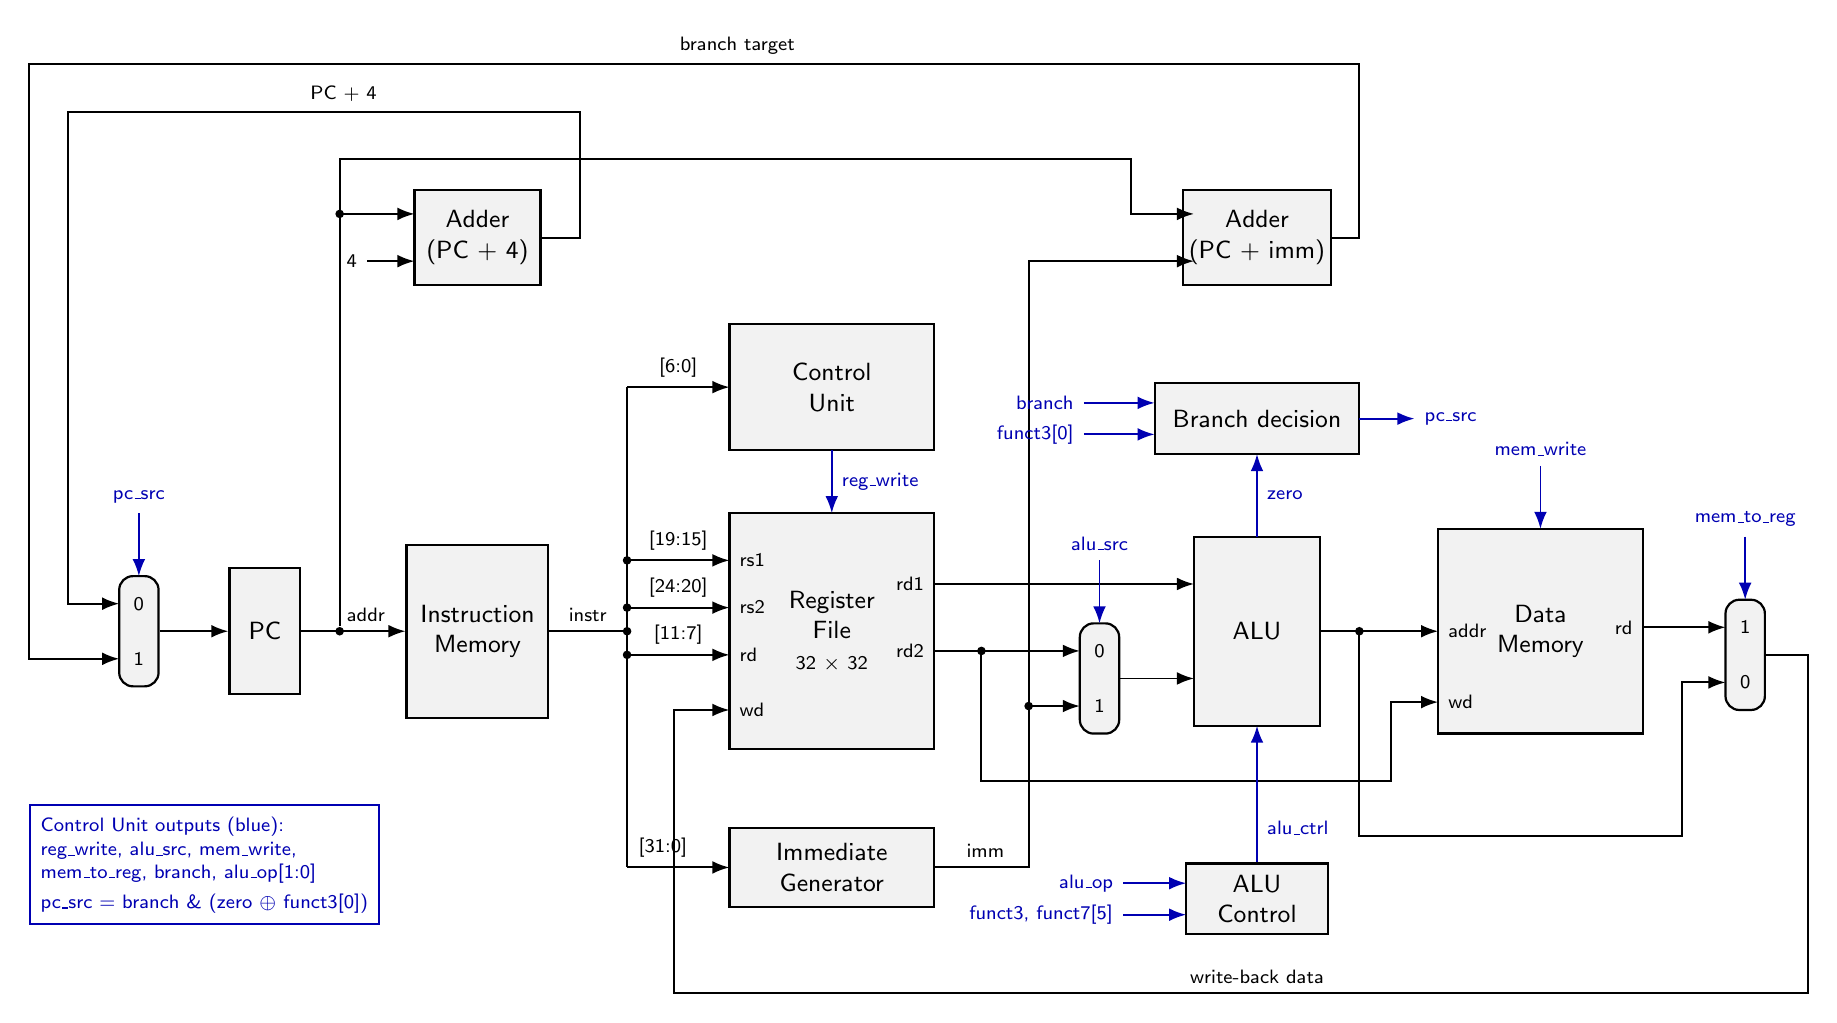
\begin{tikzpicture}[>=Latex, font=\sffamily\small, line width=0.7pt,
  blk/.style={draw, thick, fill=gray!10, align=center, inner sep=2pt},
  mux/.style={draw, thick, fill=gray!10, rounded corners=5pt,
              minimum width=0.5cm, minimum height=1.4cm, inner sep=0pt},
  ctl/.style={blue!70!black},
  dot/.style={circle, fill, inner sep=1.1pt},
  pin/.style={font=\sffamily\scriptsize}]

% ------------------------------------------------------------ blocks
\node[mux] (pcmux) at (-1.6,0) {};
\node[pin] at (-1.6,0.35) {0};  \node[pin] at (-1.6,-0.35) {1};

\node[blk, minimum width=0.9cm, minimum height=1.6cm] (pc) at (0,0) {PC};

\node[blk, minimum width=1.8cm, minimum height=2.2cm] (imem) at (2.7,0)
      {Instruction\\Memory};

\node[blk, minimum width=1.6cm, minimum height=1.2cm] (add4) at (2.7,5) {Adder\\(PC + 4)};

\node[blk, minimum width=2.6cm, minimum height=1.6cm] (ctrl) at (7.2,3.1)
      {Control\\Unit};

\node[blk, minimum width=2.6cm, minimum height=3cm] (rf) at (7.2,0) {Register\\File\\{\scriptsize 32 $\times$ 32}};

\node[blk, minimum width=2.6cm, minimum height=1cm] (imm) at (7.2,-3) {Immediate\\Generator};

\node[mux] (amux) at (10.6,-0.6) {};
\node[pin] at (10.6,-0.25) {0};  \node[pin] at (10.6,-0.95) {1};

\node[blk, minimum width=1.6cm, minimum height=2.4cm] (alu) at (12.6,0) {ALU};

\node[blk, minimum width=1.6cm, minimum height=1.2cm] (badd) at (12.6,5) {Adder\\(PC + imm)};

\node[blk, minimum width=2.6cm, minimum height=0.9cm] (bdec) at (12.6,2.7)
      {Branch decision};

\node[blk, minimum width=1.8cm, minimum height=0.9cm] (actl) at (12.6,-3.4) {ALU\\Control};

\node[blk, minimum width=2.6cm, minimum height=2.6cm] (dmem) at (16.2,0) {Data\\Memory};

\node[mux] (wmux) at (18.8,-0.3) {};
\node[pin] at (18.8,0.05) {1};  \node[pin] at (18.8,-0.65) {0};

% ------------------------------------------------------------ fetch
\draw[->] (pcmux.east) -- (pc.west);
\draw[->] (pc.east) -- node[above, pin, pos=0.62] {addr} (imem.west);
\node[dot] (pcj) at (0.95,0) {};
\draw[->] (pcj) |- (1.9,5.3);
\node[dot] at (0.95,5.3) {};
\draw[->] (0.95,5.3) |- (11.0,6.0) |- (11.8,5.3);
\draw[->] (1.3,4.7) node[left, pin] {4} -- (1.9,4.7);
% PC + 4 back to the PC mux
\draw[->] (add4.east) -- (4.0,5) |- (-2.5,6.6) |- (-1.85,0.35);
\node[pin, above] at (1.0,6.6) {PC + 4};
% branch target back to the PC mux
\draw[->] (badd.east) -- (13.9,5) |- (-3.0,7.2) |- (-1.85,-0.35);
\node[pin, above] at (6.0,7.2) {branch target};

% ------------------------------------------------------------ decode
\draw (imem.east) -- (4.6,0);
\draw (4.6,3.1) -- (4.6,-3);
\node[dot] at (4.6,0) {};
\node[dot] at (4.6,0.9) {};  \node[dot] at (4.6,0.3) {};  \node[dot] at (4.6,-0.3) {};
\node[pin, above] at (4.1,0) {instr};
\draw[->] (4.6,3.1)  -- node[above, pin] {[6:0]}   (5.9,3.1);
\draw[->] (4.6,0.9)  -- node[above, pin] {[19:15]} (5.9,0.9);
\draw[->] (4.6,0.3)  -- node[above, pin] {[24:20]} (5.9,0.3);
\draw[->] (4.6,-0.3) -- node[above, pin] {[11:7]}  (5.9,-0.3);
\draw[->] (4.6,-3)   -- node[above, pin, pos=0.35] {[31:0]}  (5.9,-3);
\node[pin, right] at (5.9,0.9)  {rs1};
\node[pin, right] at (5.9,0.3)  {rs2};
\node[pin, right] at (5.9,-0.3) {rd};
\node[pin, right] at (5.9,-1.0) {wd};
\node[pin, left]  at (8.5,0.6)  {rd1};
\node[pin, left]  at (8.5,-0.25) {rd2};

% ------------------------------------------------------------ execute
\draw[->] (8.5,0.6) -- (11.8,0.6);
\draw[->] (8.5,-0.25) -- (10.35,-0.25);
\node[dot] at (9.1,-0.25) {};
\draw[->] (9.1,-0.25) |- (14.3,-1.9) |- (14.9,-0.9);
\draw[->] (imm.east) -| (9.7,-0.95) -- (10.35,-0.95);
\node[dot] at (9.7,-0.95) {};
\draw[->] (9.7,-0.95) |- (11.8,4.7);
\node[pin, above] at (9.15,-3) {imm};
\draw[->] (amux.east) -- (11.8,-0.6);
\draw[->] (alu.east) -- (14.9,0);
\node[dot] at (13.9,0) {};
\draw[->] (13.9,0) |- (18.0,-2.6) |- (18.55,-0.65);
\node[pin, right] at (14.9,0)    {addr};
\node[pin, right] at (14.9,-0.9) {wd};
\node[pin, left]  at (17.5,0.05) {rd};

% ------------------------------------------------------------ memory / write-back
\draw[->] (17.5,0.05) -- (18.55,0.05);
\draw[->] (wmux.east) -- (19.6,-0.3) |- (5.2,-4.6) |- (5.9,-1.0);
\node[pin, above] at (12.6,-4.6) {write-back data};

% ------------------------------------------------------------ control (blue)
\begin{scope}[ctl]
  \draw[->] (7.2,2.3) -- node[right, pin] {reg\_write} (7.2,1.5);
  \draw[->] (10.6,0.9) node[above, pin] {alu\_src} -- (10.6,0.1);
  \draw[->] (16.2,2.1) node[above, pin] {mem\_write} -- (16.2,1.3);
  \draw[->] (18.8,1.2) node[above, pin] {mem\_to\_reg} -- (18.8,0.4);
  \draw[->] (-1.6,1.5) node[above, pin] {pc\_src} -- (-1.6,0.7);
  \draw[->] (actl.north) -- node[right, pin, pos=0.25] {alu\_ctrl} (12.6,-1.2);
  \draw[->] (10.9,-3.2) node[left, pin] {alu\_op} -- (11.7,-3.2);
  \draw[->] (10.9,-3.6) node[left, pin] {funct3, funct7[5]} -- (11.7,-3.6);
  \draw[->] (12.6,1.2) -- node[right, pin] {zero} (12.6,2.25);
  \draw[->] (10.4,2.9) node[left, pin] {branch} -- (11.3,2.9);
  \draw[->] (10.4,2.5) node[left, pin] {funct3[0]} -- (11.3,2.5);
  \draw[->] (13.9,2.7) -- (14.6,2.7) node[right, pin] {pc\_src};
\end{scope}

% legend
\node[draw, ctl, align=left, pin, inner sep=4pt, anchor=north west] at (-3.0,-2.2)
  {Control Unit outputs (blue):\\[1pt]
   reg\_write, alu\_src, mem\_write,\\
   mem\_to\_reg, branch, alu\_op[1:0]\\[3pt]
   pc\_src = branch \& (zero $\oplus$ funct3[0])};

\end{tikzpicture}
\end{document}
